\documentclass[conference]{IEEEtran}
%\usepackage{graphicx}
\usepackage[dvipdfmx]{graphicx}
%\usepackage{latexsym}
\usepackage{slashbox}
%\usepackage{multirow}
\usepackage{url}
\usepackage{color}
\usepackage{colortbl}
\usepackage{hhline}
\usepackage{flushend}
\usepackage{verbatim}
%\usepackage{hyperref}
\usepackage{enumerate}
\usepackage[sort&compress]{natbib}
\usepackage{subfigure}
\usepackage{framed}
%\usepackage{natbib}

\newcommand{\todo}[1]{{\color{green}{\textbf{TODO: [#1]}}}}
\newcommand{\yasu}[1]{{\color{red}{\textbf{Yasu says: [#1]}}}}
\newcommand{\emad}[1]{{\color{blue}{\textbf{[#1]}}}}
\newcommand{\Emad}[1]{{\color{blue}{\textbf{[#1]}}}}
\newcommand{\revised}[1]{{\color{red}{#1}}}
\newcommand{\para}[1]{{\color{magenta}{\textbf{This paragraph:}}} [#1]}

%\newcommand{\revised}[2]{\marginpar{\fbox{#2}}{\color{red}{#1}}}

\newcommand{\nbf}[1]{
%  \noindent{\textit{\textbf{#1}}}
  \noindent{\textbf{#1}}
}

\newcommand{\conclusionbox}[1]{%
	\vspace{2mm}
  \noindent
	\framebox[0.48\textwidth][c]{%
		\parbox[b]{0.45\textwidth}{%
			{\em #1}
		}
	}
}

% Set bibliography title
%\renewcommand\refname{REFERENCES}
%\renewcommand\bibsection{\section{\refname}}

\newcommand{\ea}{{\em et al.}}
\newcommand{\smallsection}[1]{\vspace{1mm}\noindent {\bf #1}.\hspace{2mm}}
\newcommand{\emphsection}[1]{\vspace{1mm}\noindent \underline{{\em #1}.}\hspace{2mm}}


% Reduce bibliography font size
%\def\bibfont{\normalsize} %normalsize should be default
% small or footnotesize

% Reduce space between references
%\setlength{\bibsep}{3.2pt} %3.5pt should be default


\begin{document}

\title{How Much do We Pay for Technical Debt as Interest?}

\author{
\IEEEauthorblockN{Yasutaka Kamei$^{\dag}$, Everton Maldonado$^{\dag\dag}$, Emad Shihab$^{\dag\dag}$, and Naoyasu Ubayashi$^{\dag}$}
\IEEEauthorblockA{
$^{\dag}$Principles of Software Languages Group (POSL), Kyushu University, Fukuoka, Japan\\
$^{\dag\dag}$Department of Computer Science and Software Engineering, Concordia University, Montr\'eal, Canada\\
Email: $^{\dag}$\{kamei, ubayashi\}@ait.kyushu-u.ac.jp, $^{\dag\dag}$\{e\_silvam, eshihab\}@encs.concordia.ca
}
}

% make the title area
\maketitle

% As a general rule, do not put math, special symbols or citations
% in the abstract
\begin{abstract}
abstract.
\end{abstract}

\IEEEpeerreviewmaketitle

% Here is Yasu't note
\begin{comment}
2 tomato: let's finish results (how to show)
2 tomato: read related work to get knowledge and good motivation for RQ1 and RQ2.

- slide:
2 tomato (one topic of current)
2 tomato (one topic of current)
\end{comment}

%%%%%%%%%%%%%%%%%%%%%%%%%%%%%%%%%%%%%%%%%%%%%%%%%%%%%%%%%%%
%%What is technical debt and self-admitted technical debt
Technical debt is term first coined by Cunningham in 1993 to refer to the phenomena of taking a shortcut to achieve short term development gain at the the cost of increased maintenance effort in the future \cite{Cunningham1992WPM}. The technical debt community, organized through the managing technical debt workshop \cite{Falessi2014MTD}, has studied many aspects of technical debt, including its detection \cite{Zazworka2013CSE}, impact \cite{Zazworka2011MTD}
and the appearance of technical debt in the form of code smells \cite{Fontana2012MTD}. Most recently, we developed an approach to identify technical debt from code comments, referred to as self-admitted technical debt (SATD). SATD refers to the situation where developers know that the current implementation is not optimal and write comments alerting the inadequacy of the solution.

% What people did and what is the impact of TD. What they found.
In the last few years, an increasing amount of work has focused on SATD. In particular, our prior work focused on the detection of SATD~\cite{Potdar2014ICSME} and the classification of different types of SATD and the development of datasets to enable future studies on SATD~\cite{Maldonado2015MTD}. Other work by Bavota and Russo performed an empirical study of SATD on a large number of Apache projects showed that SATD is prevalent in open source projects, is long lived and is increasing over time. A study by Wehaibi et al. \todo{cite Wehaibi} examined the impact of SATD on quality and found that SATD does not necessarily relate to more defects, however, it does make the software system more complex. 

%However, very little work focused on interest. Also, why is calculating interest difficult
Based on these prior findings, we measure and quantify the effect of SATD. In particular, we measure the amount of \emph{interest} caused by SATD. Although the metaphor of technical debt has been well studied, to the best of our knowledge, the quanitification of interest of technical debt has not been examined before. Measuring the interest if technical debt is non-trivial since it requires, in addition to the detection of the technical debt, the tracking of the debt over time and the development of a measure to accurately quantify this debt.

% What we do  and how we calculate interest
In this paper, we first propose the use of code metrics, in particular \todo{add}, as a measure of interest. We 
 
% Main contributions
The main contributions of the paper are three-fold.

\begin{itemize}
\end{itemize}

% Organization of the paper
\smallsection{Paper Organization} To purse the goal of this paper, the paper is organized as follows. 
Section \ref{background} explains the overview of defect prediction models.
Section \ref{past} revisits what challenges were in Year 2000.
%Section \ref{trends} assesses what state the research trend is in.
%Section \ref{game_changers} presents game changers, which dramatically changed perspective and direction of the studies in the field of defect prediction.
Section \ref{trends} assesses what state the research trend is in and presents some of game changers, which dramatically changed perspective and direction of the studies in the field of defect prediction.
Section \ref{challenges} highlights some key challenges for future.
Section \ref{conclusion} draws conclusions.

\section{Introduction}

<<<<<<< HEAD
\para{Describe more detail of technical debt and current problem in the domain}

Intuition and general belief indicate that ...
However, to the best of our knowledge, there is few empirical studies that 
...
Such a study would be useful ..., since ()

\para{The goal and approach of this study}

\para{Contributions}

\cite{Potdar2014ICSME}
\cite{Maldonado2015MTD}
=======
%What is technical debt and self-admitted technical debt
Technical debt is term first coined by Cunningham in 1993 to refer to the phenomena of taking a shortcut to achieve short term development gain at the the cost of increased maintenance effort in the future \cite{Cunningham1992WPM}. The technical debt community, organized through the managing technical debt workshop \cite{Falessi2014MTD}, has studied many aspects of technical debt, including its detection \cite{Zazworka2013CSE}, impact \cite{Zazworka2011MTD}
and the appearance of technical debt in the form of code smells \cite{Fontana2012MTD}. Most recently, we developed an approach to identify technical debt from code comments, referred to as self-admitted technical debt (SATD). SATD refers to the situation where developers know that the current implementation is not optimal and write comments alerting the inadequacy of the solution.

% What people did and what is the impact of TD. What they found.
In the last few years, an increasing amount of work has focused on SATD. In particular, our prior work focused on the detection of SATD~\cite{Potdar2014ICSME} and the classification of different types of SATD and the development of datasets to enable future studies on SATD~\cite{Maldonado2015MTD}. Other work by Bavota and Russo performed an empirical study of SATD on a large number of Apache projects showed that SATD is prevalent in open source projects, is long lived and is increasing over time. A study by Wehaibi et al. \todo{cite Wehaibi} examined the impact of SATD on quality and found that SATD does not necessarily relate to more defects, however, it does make the software system more complex. 

%However, very little work focused on interest. Also, why is calculating interest difficult
Based on these prior findings, we measure and quantify the effect of SATD. In particular, we measure the amount of \emph{interest} caused by SATD. Although the metaphor of technical debt has been well studied, to the best of our knowledge, the quanitification of interest of technical debt has not been examined before. Measuring the interest if technical debt is non-trivial since it requires, in addition to the detection of the technical debt, the tracking of the debt over time and the development of a measure to accurately quantify this debt.

% What we do  and how we calculate interest
In this paper, we first propose the use of code metrics, in particular \todo{add}, as a measure of interest. We 
 
% Main contributions
The main contributions of the paper are three-fold.

\begin{itemize}
\end{itemize}

% Organization of the paper
\smallsection{Paper Organization} To purse the goal of this paper, the paper is organized as follows. 
Section \ref{background} explains the overview of defect prediction models.
Section \ref{past} revisits what challenges were in Year 2000.
%Section \ref{trends} assesses what state the research trend is in.
%Section \ref{game_changers} presents game changers, which dramatically changed perspective and direction of the studies in the field of defect prediction.
Section \ref{trends} assesses what state the research trend is in and presents some of game changers, which dramatically changed perspective and direction of the studies in the field of defect prediction.
Section \ref{challenges} highlights some key challenges for future.
Section \ref{conclusion} draws conclusions.

%\para{What is technical debt?}
%
%\para{Describe more detail of technical debt and current problem in the domain}
%
%\para{The goal and approach of this study}
%
%\para{Contributions}
%
%\cite{Potdar2014ICSME}
%\cite{Maldonado2015MTD}
>>>>>>> emad

%%%%%%%%%%%%%%%%%%%%%%%%%%%%%%%%%%%%%%%%%%%%%%%%%%%%%%%%%%%
%\section{Background} \label{background}
%\emph{Prevention is better than cure.}
\para{Technical debt}

\cite{Guo2011ICSM}: they track technical debt items and access its impact (cost) among incurred, deferred and paid. That said, they focused on only one event (WebDav protocol is not supported) and 

\para{Software Evolution: We calculate interest by looking at the difference size of two versions. In other words, this work is one of lines of software evolution.}
\section{Related Work}
\para{Technical debt}

\cite{Guo2011ICSM}: they track technical debt items and access its impact (cost) among incurred, deferred and paid. That said, they focused on only one event (WebDav protocol is not supported) and 

\para{Software Evolution: We calculate interest by looking at the difference size of two versions. In other words, this work is one of lines of software evolution.}

%%%%%%%%%%%%%%%%%%%%%%%%%%%%%%%%%%%%%%%%%%%%%%%%%%%%%%%%%%%
\section{Case Study Setup} \label{sec:setup}
The goal of this study is to identify and quantify the interest of SATD in source code comments.
To conduct our case study, we use data from three open source software  projects (Apache Ant, Apache Jmeter, and JRuby). We chose these three projects, since we would like to use both of types of data sets that were used in previous studies~\cite{Maldonado2015MTD,Potdar2014ICSME} and are collected as a new one. Apache Ant and Apache Jmeter were used in previous studies, and JRuby are collected in this study. All three projects use Git as a version control system. 

\todo{Add the table that shows statistics of projects}

Table xxx shows the statistics of the projects we use in our experiments. We obtain the data sets that belong to different application domains and vary in size.

%\todo{How do we choose projects we analyze? i.e., why do we use Ant and Jmeter and do not use ArgoUML, Columba and JFreeChart? and why do we add jRuby?}

\todo{Make an overview figure to explain our approach: [Title] An overview of the design of our data extraction}

\subsection{SATD Extraction}
\smallsection{(Step 1) Extract source code files}
To perform our case study, we obtain source code files from Git repositories of three projects. We selected {\sc 1.4.0}, {\sc ANT\_170}, and {\sc v2\_10} in each JRuby, Apache Ant, and Apache jmeter as versions (tags) of which we extract SATD. The versions were released at the middle of project history. Therefore, we believe that projects elapse sufficient time for obtaining technical debt for our analysis and remain time for removing it.

\smallsection{(Step 2) Parse source code files}
After obtaining source code files, we extract the comments from them. We use JDeodorant~\cite{Tsantalis2008CSMR}, which is an open-source Eclipse plug-in, to parse the source code and extract the code comments. JDeodrant uses the Eclipse AST framework to create an Abstract Syntax Tree (AST) map of the source code. The AST map contains detailed information about the project such as: the source code comments, its type (e.g., Block, Single-line, or Javadoc), the line where each one of these comments begins and finishes. We extract the aforementioned information and store all comments as the candidate of SATD.

\smallsection{(Step 3) Filter Comments}
To reduce the number of comments we manually read, we filter comments that are less likely to be classified as SATD by utilizing several heuristics, similar to previous studies~\cite{Maldonado2015MTD}.

First, we eliminate license comments from the candidate of SATD, since we found that license comments are very not likely to contain SATD. License comments are commonly added before the declaration of the class. Since we know the line number that the class was declared we can easily check for comments that are placed before that line and remove them. In order to decrease the chances of removing a SATD comment while executing this filter we do not remove comments containing one of task-reserved words (i.e., “todo”, “fixme”, or “xxx”).

Then, we also filter Javadoc comments from the candidate of SATD, since we found that they rarely mention SATD. Based on source code comments' type provided by JDeodrant, we identify Javadoc comments. Similar to the heuristics for license comments, we do not remove Javadoc comments containing at least one of task-reserved words. To do so, we create a simple regular expression that search for the task-reserved words before removing the comment.

Then, we group consecutive single-line comments as one comment. We notice that developers sometimes make long comments, using multiple single-line comments instead of a Block comment. This characteristic can hinder the understanding of the message. When considering the case that we analyze each one of these comments independently, we may misunderstand the message because each of them would be incomplete and lose the meaning.

Finally, we filter the comments that conduct {\it comment out} source code from the candidate of SATD. While commented source code may show the code that is currently not being used or the code that was used for debugging, it may not include any developer's comments. Therefore, the commented source code is less likely to be classified as SATD. We remove commented source code using a simple regular expression that captures typical Java code structures.

Table xxx shows the number of comments that are filtered by the heuristics we used. The heuristics significantly reduces the number of comments in our dataset and helps us focus on the most applicable and insightful comments. 

\todo{add a table that shows the number of comments that are filtered by several heuristics}

\smallsection{(Step 4) Manual Classification}
To extract SATD, the xxx author manually classified all comments into SATD or not.
The xxx author who made the classification has more than 8 years of experience working in the industry as a software engineer, during this time he designed, implemented and maintained several programs using, in particular the Java programming language. He developed solid skills in object orientated programming and design patterns. We consider that these qualifications provide the necessary background to conduct the manual classification of the comments.

\subsection{Interest Extraction} \label{subsec:interest}

\smallsection{(Step 1) Identify two versions that introduce and remove technical debt}
By tracing the comments including SATD across versions in Git repositories, we identify two versions that introduce and remove them. To trace the comments, we obtain patches between two versions over all versions for each file that includes technical debt. Then, we check each patch about whether or not technical debt is introduced and removed. 

\smallsection{(Step 2) Measure metrics}
To calculate interest, we measure product metrics from two versions detected in Step 1 using {\sc Understand}~\cite{Understand}. We choose all metrics that are available at the method-level in {\sc Understand}.

\smallsection{(Step 3) Calculate interest}
There are many ways to calculate interest of SATD. Therefore, in this study, we consider the relative size of metric values between two versions as interest, since that approach is simple and intuitive. For example, if arbitrary metric values in introduced and removed versions are 10 and 20, the relative size is 100 (= (20-10)/10 * 100 ).
If we cannot find the version that removes SATD, 
we use the latest release version of each system. 

While the paper tackles the research topic that accelerates a new research direction (i.e., quantifying interest of SATD), it also has the weakness of our current approach. We elaborate on the weakness of our current approach in Section \todo{xxx}.

%%%%%%%%%%%%%%%%%%%%%%%%%%%%%%%%%%%%%%%%%%%%%%%%%%%%%%%%%%%
\section{Results}
\subsection{RQ1: Can we quantify interest of technical debt at the method-level?}
\smallsection{Motivation}
To alleviate the impact of technical debt, there are several previous studies on understanding SATD (e.g., the detection of technical debt~\cite{Potdar2014ICSME,Zazworka2013EASE} and the impact of SATD on software quality~\cite{Wehaibi2016SANER}).
However, there are few empirical studies that quantify interest of SATD.
Therefore, we would like to know how we can understand interest using our method explained in Section \ref{subsec:interest}

\smallsection{Approach}
%\para{We calculate the interest.}
To calculate interest of SATD, we follow the approach we explained in Section \ref{sec:setup}.

\smallsection{Results}
We find that there are high correlations between LOC and the other product metrics except Fan-In. 
From the highly correlated metrics, we choose LOC as metrics to calculate interest, similar to previous work that considers effort in the domain of defect prediction~\cite{Kamei2010ICSM,Kamei2013TSE}. We assume that developers spend more effort to check larger methods before modifying the methods. Eventually, we show our results using two product metrics (i.e., LOC and Fan-In).

Table \ref{tab:statistic} shows the number of SATD and the percentage of the technical debt that has positive interest in all technical debt. 

Figure \ref{fig:dist} shows that the distribution of interest. X
\para{Put the distribution of interest?}

\begin{table}[tb]
  \caption{Statistic interest of SATD}
  \label{tab:statistic}
  \centering

  \begin{tabular}{cl|r|rrr}
  \hline
      &  Project & Positive Rate & All & Positive & Negative \\
  \hline
        & Ant    & 38.0\% &  71 &  27  &  20 \\
   LOC  & JMeter & 44.2\% & 181 &  80  &  25 \\
        & JRuby  & 32.6\% & 236 &  77  &  59 \\
  \hline
        & Ant    & 30.9\% &  68 &  21  &  13 \\
Fan-In  & JMeter & 42.2\% & 161 &  68  &  13 \\
        & JRuby  & 30.3\% & 231 &  70  &  37 \\
  \hline
  \end{tabular}
\end{table}

%-----------------------------------------------------------------------
\begin{figure*}[!t]
  \begin{center}
  \scalebox{0.95}{
  \begin{tabular}{ccc}
    \subfigure[Ant (LOC)]{ 
      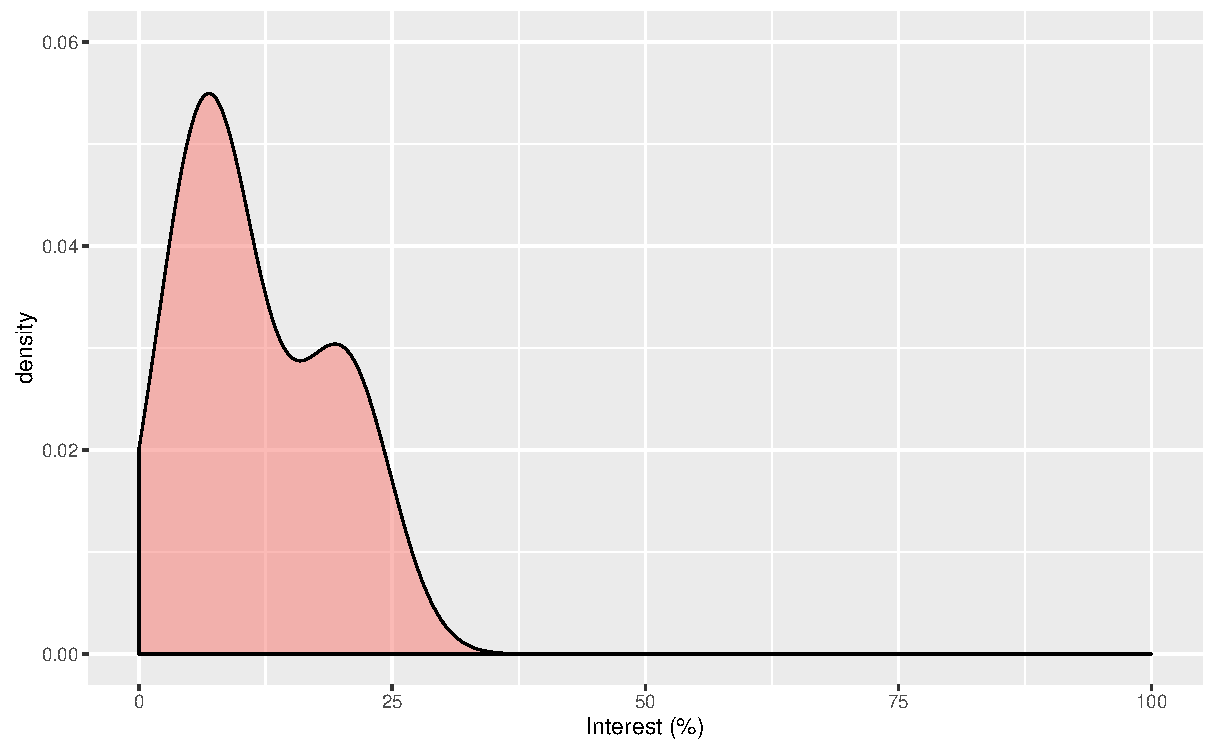
\includegraphics[width=.33\textwidth]{figures/rq1-ant}
    }
    \subfigure[JMeter (LOC)]{ 
      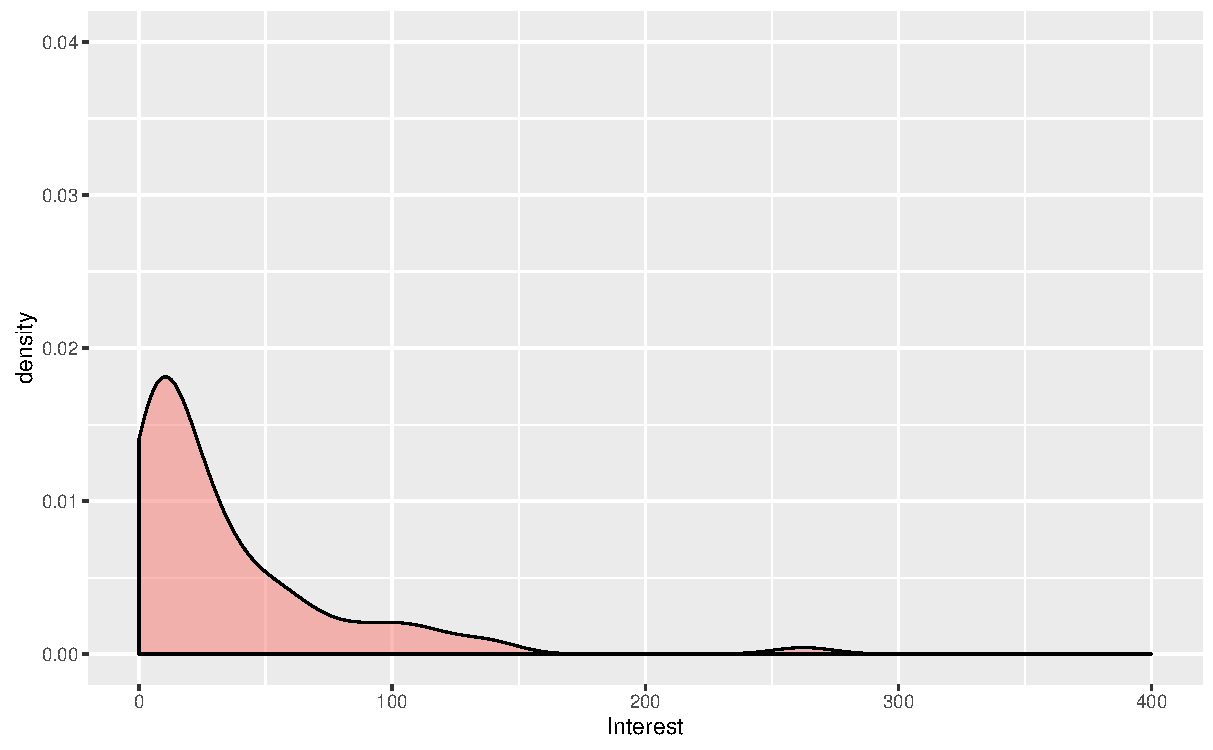
\includegraphics[width=.33\textwidth]{figures/rq1-jmeter}
    }
    \subfigure[JRuby (LOC)]{
      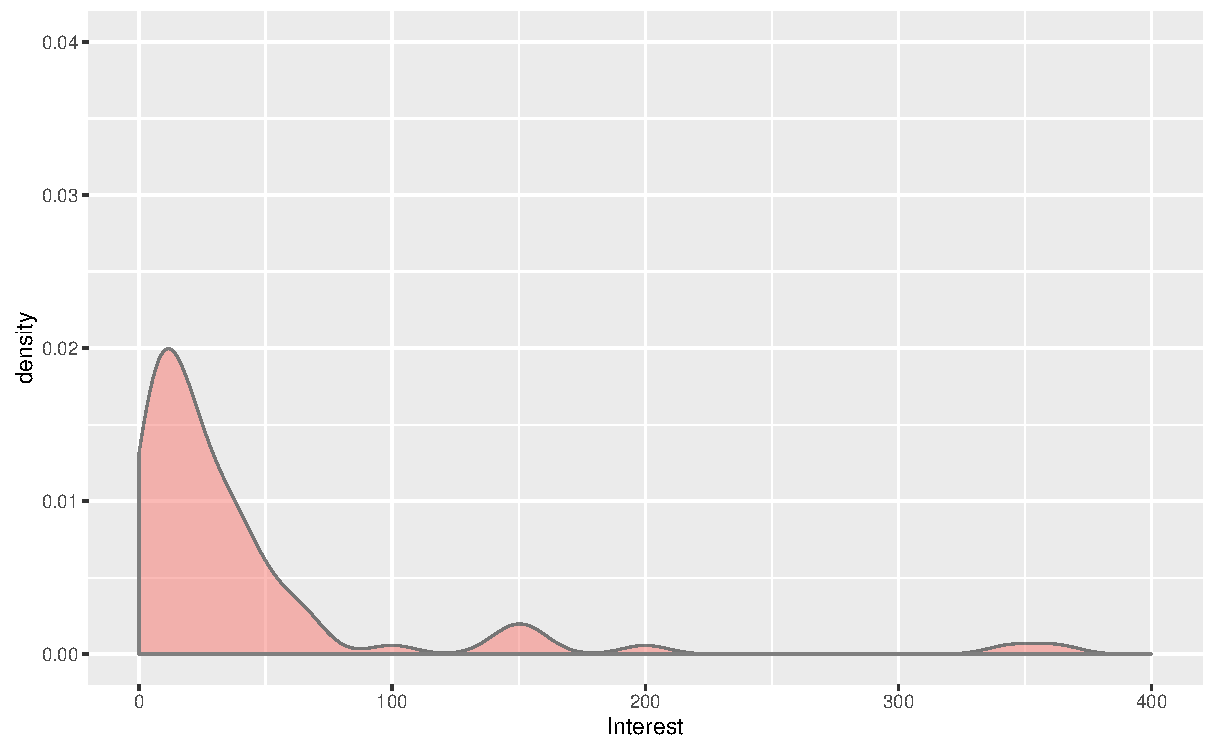
\includegraphics[width=.33\textwidth]{figures/rq1-jruby}
    }
  \end{tabular}
  }
  \scalebox{0.95}{
  \begin{tabular}{ccc}
    \subfigure[Ant (Fan-In)]{ 
      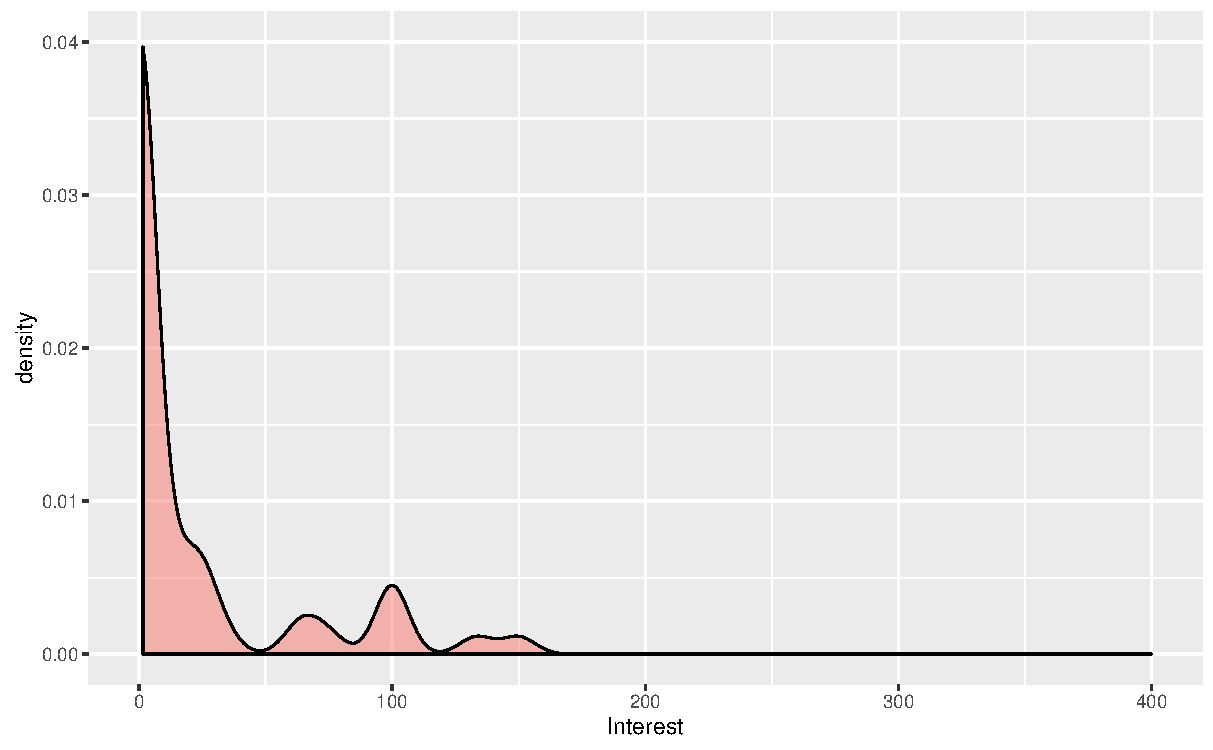
\includegraphics[width=.33\textwidth]{figures/rq1-ant-fanin}
    }
    \subfigure[JMeter (Fan-In)]{ 
      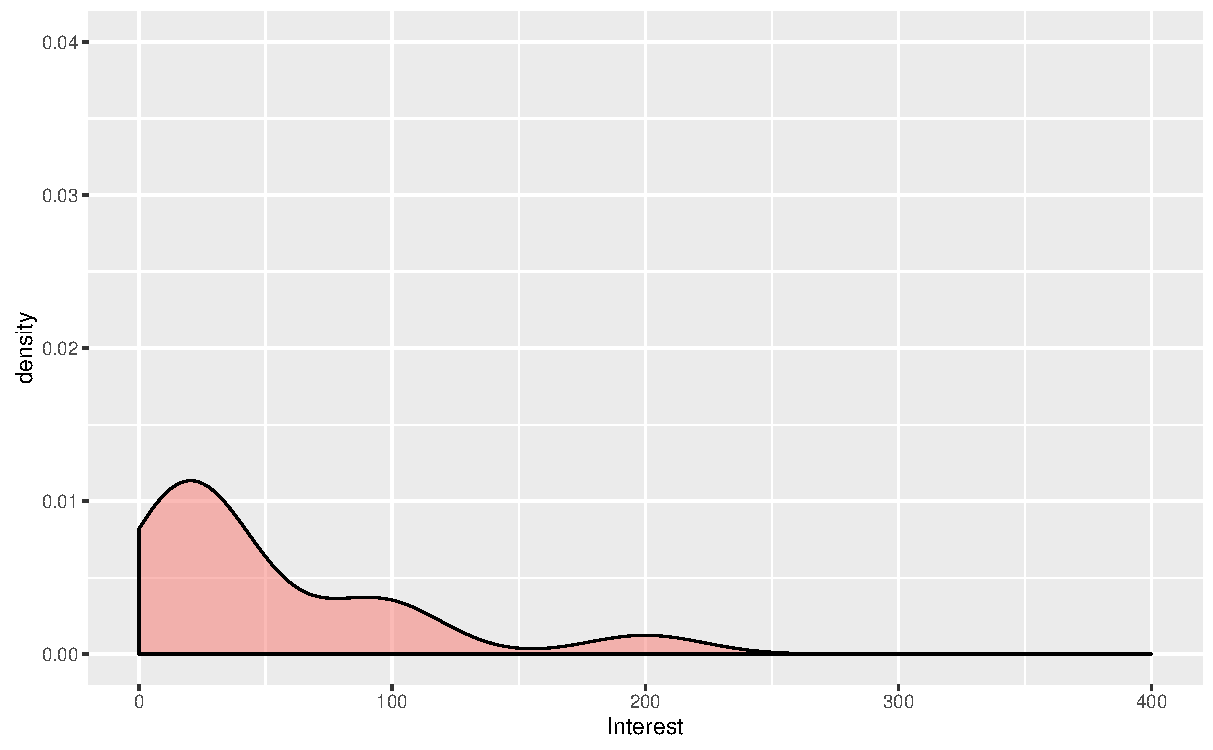
\includegraphics[width=.33\textwidth]{figures/rq1-jmeter-fanin}
    }
    \subfigure[JRuby (Fan-In)]{
      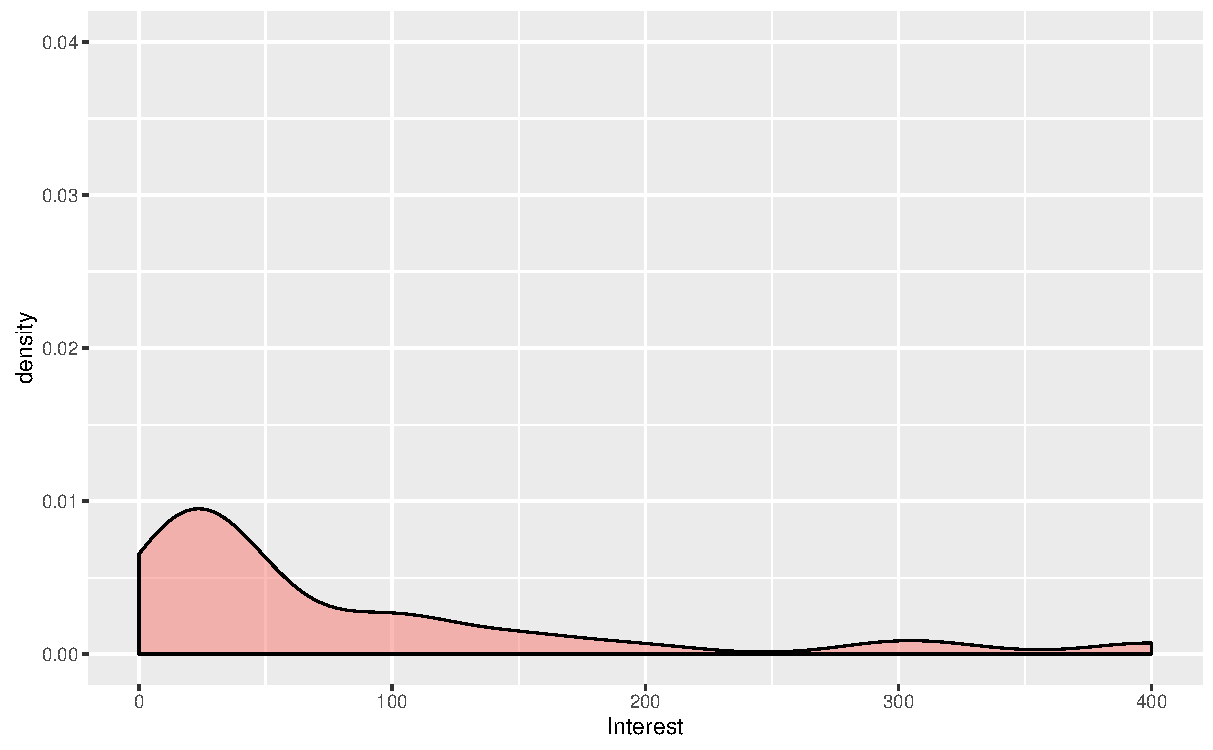
\includegraphics[width=.33\textwidth]{figures/rq1-jruby-fanin}
    }
  \end{tabular}
  }
  \caption{(RQ1) The results of distribution of interest.}
  \label{fig:dist}
  \end{center}
\end{figure*}
%-----------------------------------------------------------------------


\conclusionbox{Result of RQ1: 22\%-36\% of technical debt has positive interest.}

\subsection{RQ2: Does the interest differ based on the type of technical debt?}
\smallsection{Motivation}
There are several type of technical debt such as defect technical debt and design technical debt. 
To better understand the interest, we would like to analayze ...

\smallsection{Approach}
We classify technical debt into categories and calculate interest in each category.

\smallsection{Results}
Table X shows the number and the percentage of technical debt. Among three projects, jruby only includes more than one category that has more than 10\% of technical debt methods. Therefore, we decided to use jruby in RQ2.

\para{we report same things in RQ1.}  

%-----------------------------------------------------------------------
\begin{figure}
  \centering
  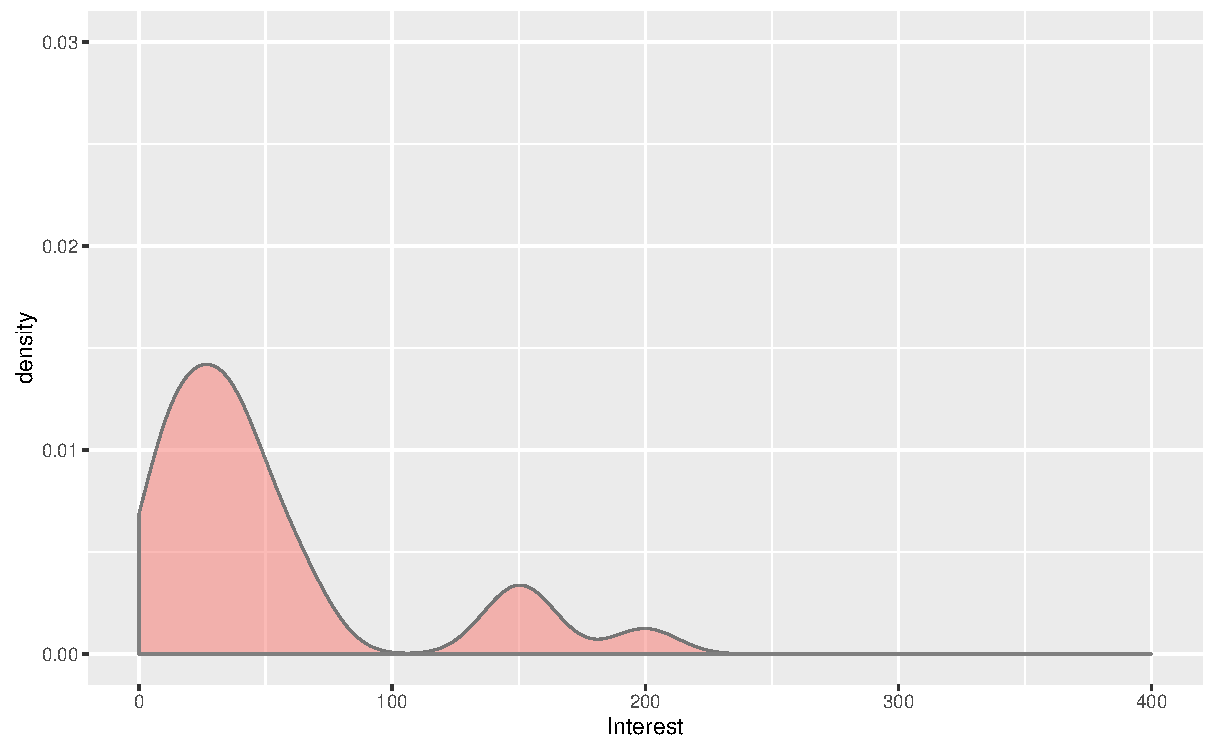
\includegraphics[width=.45\textwidth]{figures/rq2-defect}
  \caption{Adding a Repository in Commit Guru \label{fig:guru1}}
\end{figure}
\begin{figure}
  \centering
  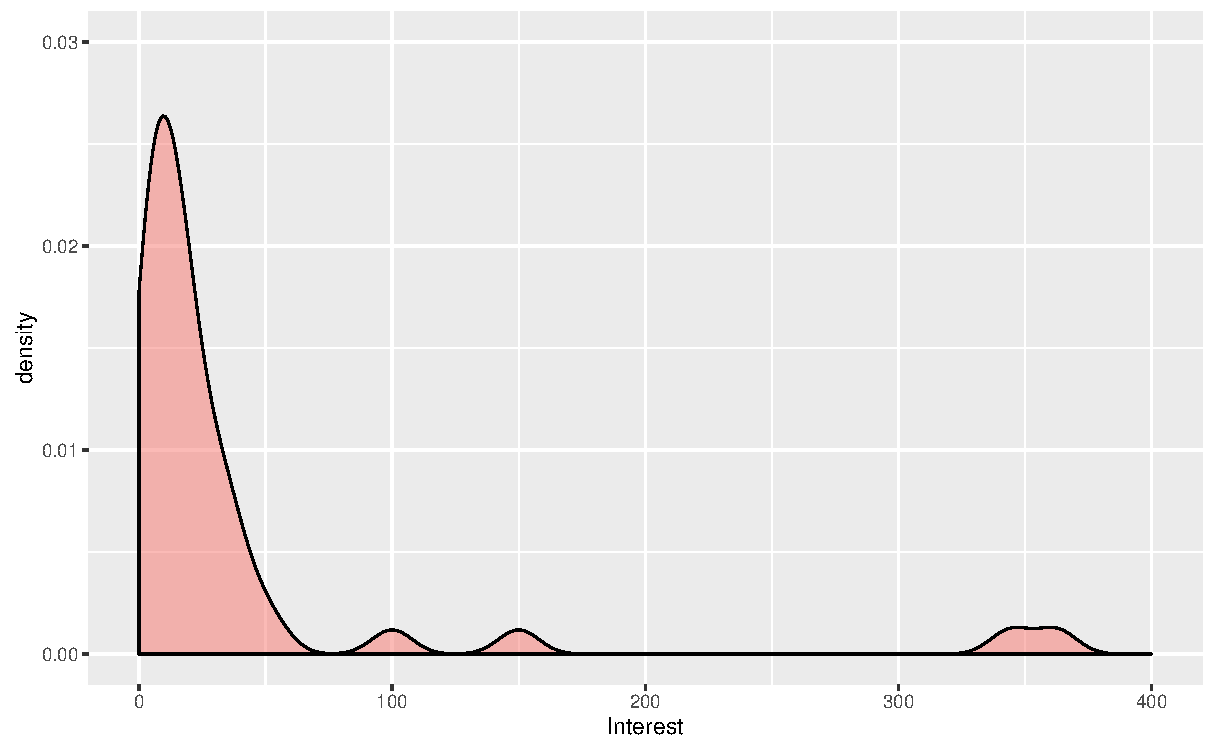
\includegraphics[width=.45\textwidth]{figures/rq2-design}
  \caption{Adding a Repository in Commit Guru \label{fig:guru1}}
\end{figure}
\begin{figure}
  \centering
  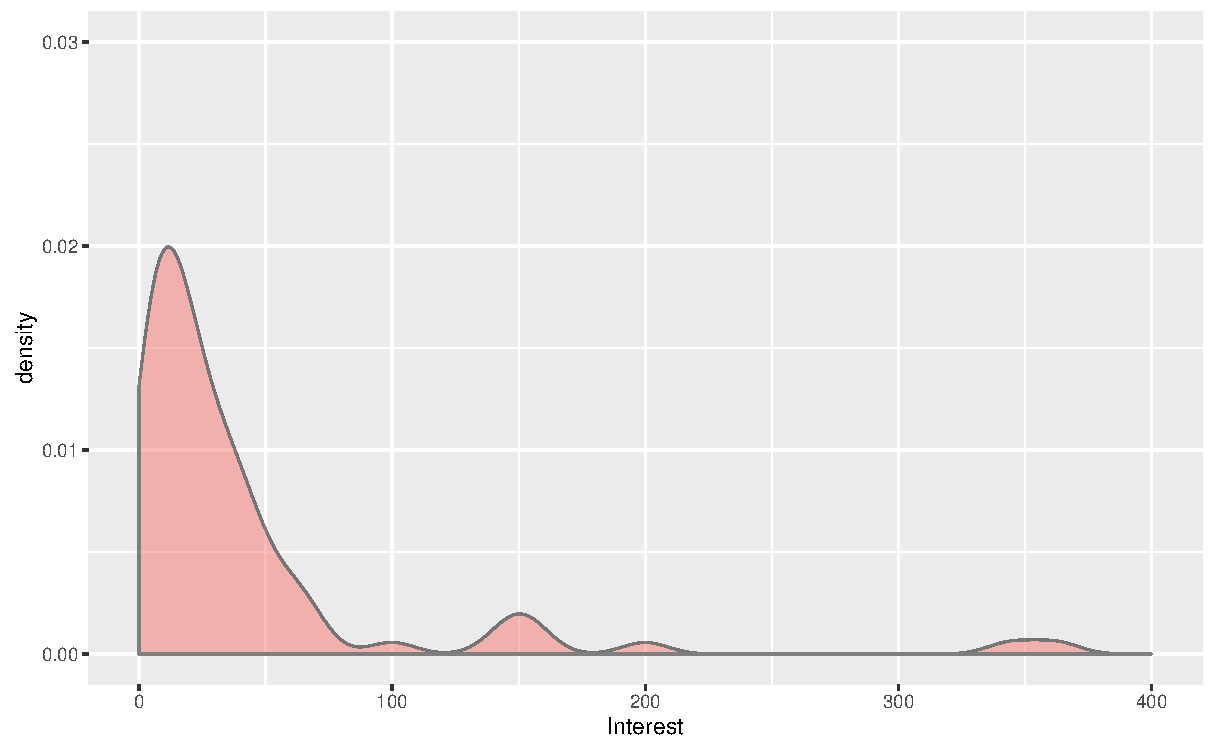
\includegraphics[width=.45\textwidth]{figures/rq2-requirement}
  \caption{Adding a Repository in Commit Guru \label{fig:guru1}}
\end{figure}
%-----------------------------------------------------------------------


\conclusionbox{Result of RQ2}

\subsection{RQ3: manual analysis}
\smallsection{Motivation}

\smallsection{Approach}

\smallsection{Results}

\conclusionbox{Result of RQ3}

\section{Discussion}
\para{Put additional analysis when considering time period.}

\para{Put additional analysis when considering other metrics (fan-in).}

\para{Put additional analysis when comparing the non-technical deb methods.}

\para{Put the analysis for showing the method that includes more than one technical debt in one version.}

%%%%%%%%%%%%%%%%%%%%%%%%%%%%%%%%%%%%%%%%%%%%%%%%%%%%%%%%%%%
\section{Threat to Validity}

\smallsection{Construct Validity}

\smallsection{Internal Validity}
\para{Technical debt is classified by one person.}

\smallsection{External Validity}

%%%%%%%%%%%%%%%%%%%%%%%%%%%%%%%%%%%%%%%%%%%%%%%%%%%%%%%%%%%
\section{Conclusion}
%\section{Conclusion} \label{conclusion}
%\section{Conclusion} \label{conclusion}
%\section{Conclusion} \label{conclusion}
%\input{conclusion.tex}
\para{Summary of this work.}

\smallsection{Future direction}

\begin{itemize}
\item \todo{Discuss how to calculate interest.}
\item  There are several type of technical debt such as defect technical debt and design technical debt.
The previous study~\cite{Maldonado2015MTD} shows that the percentage of technical debt varies depending on the type of technical debt and the studied systems. For example, the projects that have limited time to develop features are likely to leave comments of features that need to be implemented in the future. 
To better understand the interest, we would like to analyze the interest per type of technical debt.
\item  The interest varies among technical debt. If we can understand the reason why some of technical debt has large interest, we can make use of such insights for future development. Therefore, we would like to manually investigate why some of technical debt has large interest.
\item Generally speaking, software systems are always evolving over time for implementing new functionality and fixing defects~\cite{xxx}.
Therefore, even if the size of technical debt increases, it is not clear about how the nature of software evaluation affects the interest of technical debt.
We would like to compare the impact of software evolution on methods in two groups of SATD v.s. non-SATD.
\item To operationalize our findings, we also built a tool that is able to identify and assign an interest rate to all SATD instances in a project. Our tool is publicly available and can be used by practitioners to prioritize the most impacting (i.e., highest interest) SATD.
\end{itemize}

\para{Summary of this work.}

\smallsection{Future direction}

\begin{itemize}
\item \todo{Discuss how to calculate interest.}
\item  There are several type of technical debt such as defect technical debt and design technical debt.
The previous study~\cite{Maldonado2015MTD} shows that the percentage of technical debt varies depending on the type of technical debt and the studied systems. For example, the projects that have limited time to develop features are likely to leave comments of features that need to be implemented in the future. 
To better understand the interest, we would like to analyze the interest per type of technical debt.
\item  The interest varies among technical debt. If we can understand the reason why some of technical debt has large interest, we can make use of such insights for future development. Therefore, we would like to manually investigate why some of technical debt has large interest.
\item Generally speaking, software systems are always evolving over time for implementing new functionality and fixing defects~\cite{xxx}.
Therefore, even if the size of technical debt increases, it is not clear about how the nature of software evaluation affects the interest of technical debt.
We would like to compare the impact of software evolution on methods in two groups of SATD v.s. non-SATD.
\item To operationalize our findings, we also built a tool that is able to identify and assign an interest rate to all SATD instances in a project. Our tool is publicly available and can be used by practitioners to prioritize the most impacting (i.e., highest interest) SATD.
\end{itemize}

\para{Summary of this work.}

\smallsection{Future direction}

\begin{itemize}
\item \todo{Discuss how to calculate interest.}
\item  There are several type of technical debt such as defect technical debt and design technical debt.
The previous study~\cite{Maldonado2015MTD} shows that the percentage of technical debt varies depending on the type of technical debt and the studied systems. For example, the projects that have limited time to develop features are likely to leave comments of features that need to be implemented in the future. 
To better understand the interest, we would like to analyze the interest per type of technical debt.
\item  The interest varies among technical debt. If we can understand the reason why some of technical debt has large interest, we can make use of such insights for future development. Therefore, we would like to manually investigate why some of technical debt has large interest.
\item Generally speaking, software systems are always evolving over time for implementing new functionality and fixing defects~\cite{xxx}.
Therefore, even if the size of technical debt increases, it is not clear about how the nature of software evaluation affects the interest of technical debt.
We would like to compare the impact of software evolution on methods in two groups of SATD v.s. non-SATD.
\item To operationalize our findings, we also built a tool that is able to identify and assign an interest rate to all SATD instances in a project. Our tool is publicly available and can be used by practitioners to prioritize the most impacting (i.e., highest interest) SATD.
\end{itemize}

\para{Summary of this work.}

\section*{Acknowledgment}
This research was partially supported by JSPS KAKENHI Grant Numbers 15H05306.

\bibliographystyle{abbrv}
%\bibliographystyle{IEEEtranN}
\bibliography{reference}


\end{document}

